\begin{figure*}
\centering
\begin{tabular}{lc}
& \small Total elements \\
\rotatebox[origin=c]{90}{\small Threads \kern 1em} & {\pgfplotstabletypeset[
    font=\footnotesize,
    color cells={
        min = 1.44, 
        max = 2.5},
    /pgfplots/colormap = {whitered}{
        rgb255(0cm) = (120, 40, 40); rgb255(1cm) = (200, 200, 200)
    },
    /color cells/textcolor/.initial = {white},
    every head row/.style={
    typeset cell/.code={%% add the word 'Rank'...
    \ifnum\pgfplotstablecol=\pgfplotstablecols%
    \pgfkeyssetvalue{/pgfplots/table/@cell content}{1600 \\}%
    \else%
    \ifnum\pgfplotstablecol=1%
    \pgfkeyssetvalue{/pgfplots/table/@cell content}{&}%
    \else%
    \ifnum\pgfplotstablecol=2%
    \pgfkeyssetvalue{/pgfplots/table/@cell content}{ 9 &}%
    \else%
    \ifnum\pgfplotstablecol=3%
    \pgfkeyssetvalue{/pgfplots/table/@cell content}{ 16 &}%
    \else%
    \ifnum\pgfplotstablecol=4%
    \pgfkeyssetvalue{/pgfplots/table/@cell content}{ 25 &}%
    \else%
    \ifnum\pgfplotstablecol=5%
    \pgfkeyssetvalue{/pgfplots/table/@cell content}{ 36 &}%
    \else%
    \ifnum\pgfplotstablecol=6%
    \pgfkeyssetvalue{/pgfplots/table/@cell content}{ 49 &}%
    \else%
    \ifnum\pgfplotstablecol=7%
    \pgfkeyssetvalue{/pgfplots/table/@cell content}{ 64 &}%
    \else%
    \ifnum\pgfplotstablecol=8%
    \pgfkeyssetvalue{/pgfplots/table/@cell content}{ 100 &}%
    \else%
    \ifnum\pgfplotstablecol=9%
    \pgfkeyssetvalue{/pgfplots/table/@cell content}{ 144 &}%
    \else%
    \ifnum\pgfplotstablecol=10%
    \pgfkeyssetvalue{/pgfplots/table/@cell content}{ 196 &}%
    \else%
    \ifnum\pgfplotstablecol=11%
    \pgfkeyssetvalue{/pgfplots/table/@cell content}{ 225 &}%
    \else%
    \ifnum\pgfplotstablecol=12%
    \pgfkeyssetvalue{/pgfplots/table/@cell content}{ 400 &}%
    \else%
    \ifnum\pgfplotstablecol=13%
    \pgfkeyssetvalue{/pgfplots/table/@cell content}{ 441 &}%
    \else%
    \ifnum\pgfplotstablecol=14%
    \pgfkeyssetvalue{/pgfplots/table/@cell content}{ 576 &}%
    \else%
    \ifnum\pgfplotstablecol=15%
    \pgfkeyssetvalue{/pgfplots/table/@cell content}{ 784 &}%
    \else%
    \ifnum\pgfplotstablecol=16%
    \pgfkeyssetvalue{/pgfplots/table/@cell content}{ 900 &}%
    \else%
    \ifnum\pgfplotstablecol=17%
    \pgfkeyssetvalue{/pgfplots/table/@cell content}{ 1225 &}%
    \else%
    \pgfkeyssetvalue{/pgfplots/table/@cell content}{1600 \\}%
    \fi\fi\fi\fi\fi\fi\fi\fi\fi\fi\fi\fi\fi\fi\fi\fi\fi\fi%
    }%%
    },
    col sep = comma,
    columns/0/.style={reset styles}
]{./data/tts}} \\
\end{tabular}
\caption{Time to solution (seconds) given fixed problem size for various 
    element and thread configurations on a single Xeon E5-2690 node.}
\end{figure*}


%,9,16,25,36,49,64,100,144,196,225,400,441,576,784,900,1225,1600

\section{Performance evaluation in shared memory}
\noindent 
The most performant PDE solvers for large-scale problems are increasingly based on GPUs, but often do so by constraining properties of system, such as enforcing FPD-ness in the case of iterative solvers. We show that the hybrid SBP-SAT method can be compute similarly large problems with fewer constraints on the CPU.  

\subsection{Evaluation}

\begin{figure}
\centering
\begin{subfigure}[b]{1\columnwidth}
\centering
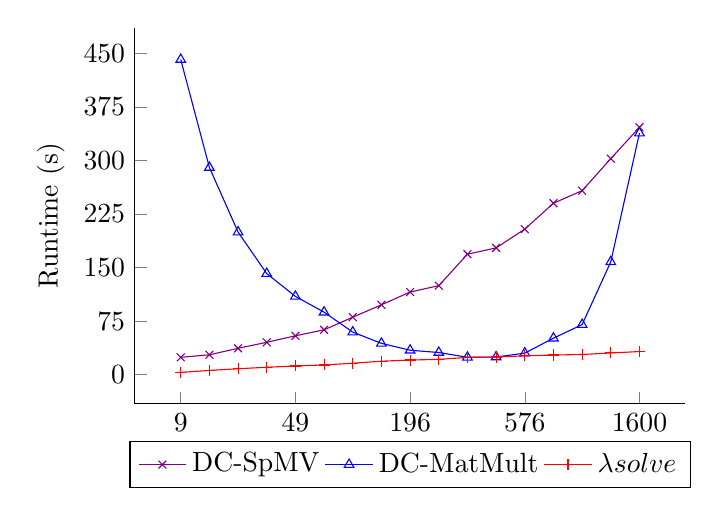
\begin{tikzpicture}
    \begin{axis}[
        legend style={
            at={(0.5,-0.1)},
            anchor=north,legend columns=-1},
        height=2.5in,
        width=3.375in,
        axis x line*=bottom,
        axis y line*=left,
        symbolic x coords = {9, 16, 25, 36, 49, 64, 100, 144, 196, 225, 400, 441, 576, 784, 900, 1225, 1600},
        xtick = {9, 49, 196, 576, 1600},
        ytick distance=75,
        domain = 9:1600,
        range = 0:450,
        xlabel={Elements},
        ylabel={Runtime (s)}]
        \addplot[
            mark=x,
            color=violet] coordinates {
                (9, 24.325156)
            	(16, 27.834308) 
            	(25, 36.956056)
            	(36, 45.347331)
            	(49, 54.437361)
            	(64, 62.814148)
            	(100, 80.488467)
            	(144, 97.845769)             	 
            	(196, 115.743751) 
            	(225, 124.628909) 
            	(400, 168.691478) 
            	(441, 177.584231) 
            	(576, 203.812683) 
            	(784, 240.088173) 
            	(900, 257.634123) 
            	(1225, 302.521926)
            	(1600, 346.441605)		
            };                
        \addplot[
            mark=triangle,
            color=blue] coordinates {
                (9, 441.321048)
            	(16, 290.10575)
            	(25, 199.676772)
            	(36, 141.542836)
            	(49, 109.624197)
            	(64, 87.516978)
            	(100, 59.597739)
            	(144, 43.86835)             	 
            	(196, 34.223977) 
            	(225, 31.043727) 
            	(400, 24.364813) 
            	(441, 24.756918) 
            	(576, 30.185676) 
            	(784, 51.117228) 
            	(900, 70.110809) 
            	(1225, 158.006306)
            	(1600, 338.225247)		
            };
        \addplot[
            mark=+,
            color=red] coordinates {
                (9, 3.186158)
            	(16, 5.987428)
            	(25, 8.304203)
            	(36, 10.420171)
            	(49, 12.213909)
            	(64, 13.637598)
            	(100, 16.047212)
            	(144, 18.873235)             	 
            	(196, 20.515413) 
            	(225, 21.414372)
            	(400, 24.244844) 
            	(441, 24.780033) 
            	(576, 26.379761) 
            	(784, 27.517695) 
            	(900, 28.265589) 
            	(1225, 30.447891)
            	(1600, 32.383344)		
            };
        \addlegendentry{DC-SpMV}
        \addlegendentry{DC-MatMult}
        \addlegendentry{$\symbf{\lambda} \text{ solve}$} 
    \end{axis}
\end{tikzpicture}
\end{subfigure}
\begin{subfigure}[b]{1\columnwidth}
\centering
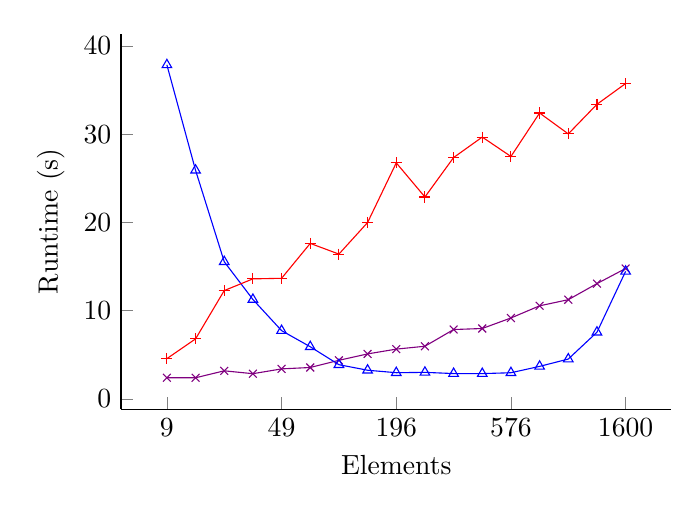
\begin{tikzpicture}
    \begin{axis}[
        height=2.5in,
        width=3.375in,
        axis x line*=bottom,
        axis y line*=left,
        symbolic x coords = {9, 16, 25, 36, 49, 64, 100, 144, 196, 225, 400, 441, 576, 784, 900, 1225, 1600},
        xtick = {9, 49, 196, 576, 1600},
        ytick distance=10,
        domain = 9:1600,
        range = 0:40,
        xlabel={Elements},
        ylabel={Runtime (s)}]
        \addplot[
            mark=x,
            color=violet] coordinates {
                (9, 2.397702)
                (16, 2.394517) 
                (25, 3.180994)
                (36, 2.855465)
                (49, 3.40153)
                (64, 3.558418)
                (100, 4.372501)
                (144, 5.095191)                  
                (196, 5.641578) 
                (225, 5.964769) 
                (400, 7.857667) 
                (441, 7.976037) 
                (576, 9.166833) 
                (784, 10.545802) 
                (900, 11.238055) 
                (1225, 13.058728)
                (1600, 14.773929)       
            };                            
        \addplot[
            mark=triangle,
            color=blue] coordinates {
                (9, 37.839475)
                (16, 25.899214)
                (25, 15.539969)
                (36, 11.263805)
                (49, 7.735455)
                (64, 5.908895)
                (100, 3.875921)
                (144, 3.248426)                  
                (196, 2.967249) 
                (225, 3.007436) 
                (400, 2.871237) 
                (441, 2.866318) 
                (576, 2.963138) 
                (784, 3.684828) 
                (900, 4.5139599) 
                (1225, 7.553876)
                (1600, 14.450906)       
            };     
        \addplot[
            mark=+,
            color=red] coordinates {
                (9, 4.562236)
                (16, 6.799783)
                (25, 12.272318)
                (36, 13.599193)
                (49, 13.662346)
                (64, 17.617201)
                (100, 16.404489)
                (144, 19.981687)                 
                (196, 26.740117) 
                (225, 22.875268)
                (400, 27.343023) 
                (441, 29.659641) 
                (576, 27.462272) 
                (784, 32.388184) 
                (900, 30.020221) 
                (1225, 33.37332)
                (1600, 35.725706)       
            };

    \end{axis}
\end{tikzpicture}
\end{subfigure}
\caption{Runtime of routines that significantly contribute to the overall
    runtime for various element configurations. 1 thread (top) and 28 
    threads (bottom). }
\end{figure}


\subsection{MatMult Analysis}

\begin{figure}[!b]
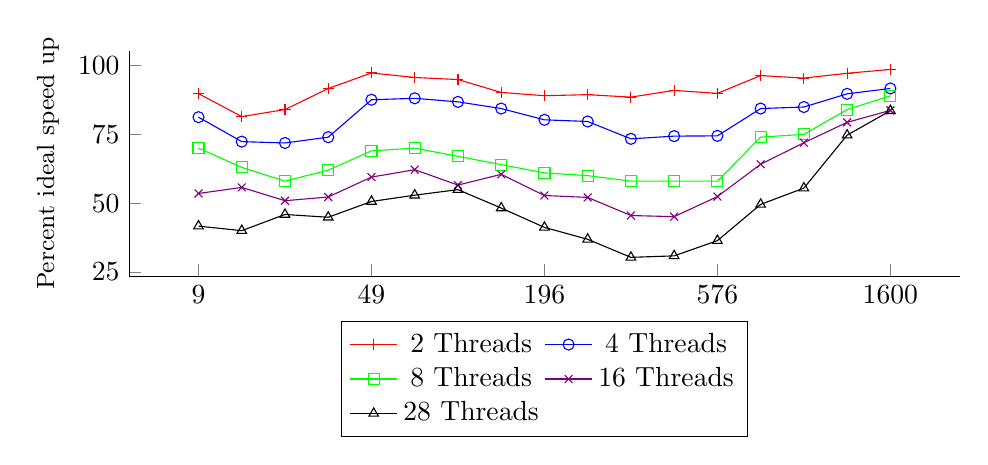
\begin{tikzpicture}
    \begin{axis}[
	    legend style={
            at={(0.5,-0.2)},
            anchor=north,
            legend columns=2},
        height=1.75in,
        width=\columnwidth,
        axis x line*=bottom,
        axis y line*=left,
        symbolic x coords = {9, 16, 25, 36, 49, 64, 100, 144, 196, 225, 400, 441, 576, 784, 900, 1225, 1600},
        xtick = {9, 49, 196, 576, 1600},
        ytick distance=25.,
        domain = 9:1600,
        range = 0:1,
        xlabel={\small Elements ($\ell^2$)},
        ylabel={\small Percent ideal speed up}]
	\addplot[
        mark=+,
        color=red] coordinates { 
            (9,89.80772783)
			(16,81.44809896)
			(25,84.01265431)
			(36,91.65362266)
			(49,97.3178835)
			(64,95.66418795)
			(100,94.91731162)
			(144,90.23017479)
			(196,89.04560603)
			(225,89.42606936)
			(400,88.52873523)
			(441,90.96957938)
			(576,89.89312948)
			(784,96.362808)
			(900,95.4433221)
			(1225,97.19841906)
			(1600,98.58183248)};
	\addlegendentry{2 Threads}
    \addplot[
        mark=o,
        color=blue] coordinates {
            (9,81.24280595)
			(16,72.35409511)
			(25,71.87422205)
			(36,73.97099956)
			(49,87.57828937)
			(64,88.09522093)
			(100,86.80642458)
			(144,84.38193744)
			(196,80.28113664)
			(225,79.68067235)
			(400,73.36438178)
			(441,74.36115039)
			(576,74.44781356)
			(784,84.37458405)
			(900,84.94134329)
			(1225,89.72037773)
			(1600,91.68107848)};
	\addlegendentry{4 Threads}
	\addplot[
        mark=square,
        color=green] coordinates {
            (9,70)
			(16,63)
			(25,58)
			(36,62)
			(49,69)
			(64,70)
			(100,67)
			(144,64)
			(196,61)
			(225,60)
			(400,58)
			(441,58)
			(576,58)
			(784,74)
			(900,75)
			(1225,84)
			(1600,89)};
	\addlegendentry{8 Threads}
	\addplot[
        mark=x,
        color=violet] coordinates {
            (9,53.52149343)
			(16,55.72203392)
			(25,50.88135743)
			(36,52.24498021)
			(49,59.47561476)
			(64,62.16044819)
			(100,56.57392172)
			(144,60.4699287)
			(196,52.77826458)
			(225,52.08890179)
			(400,45.50386094)
			(441,45.10367777)
			(576,52.38086479)
			(784,64.13954692)
			(900,71.95346234)
			(1225,79.35939415)
			(1600,83.71552989)};
	\addlegendentry{16 Threads}			
	\addplot[
        mark=triangle,
        color=black] coordinates {
            (9,41.65350074)
			(16,40.00476479)
			(25,45.89013843)
			(36,44.87916193)
			(49,50.6130524)
			(64,52.89663054)
			(100,54.91573947)
			(144,48.23033634)
			(196,41.1925286)
			(225,36.86544072)
			(400,30.30651572)
			(441,30.84708825)
			(576,36.38237089)
			(784,49.5441113)
			(900,55.47142684)
			(1225,74.70446109)
			(1600,83.58972861)};
	\addlegendentry{28 Threads}
    \end{axis}
\end{tikzpicture}
\caption{Performance of the decomposed MatMult kernel on a fixed problem size (705600 grid points) for various thread counts and total elements.}
\end{figure}
										
													


%\begin{mcfigure}
%	\centering
%	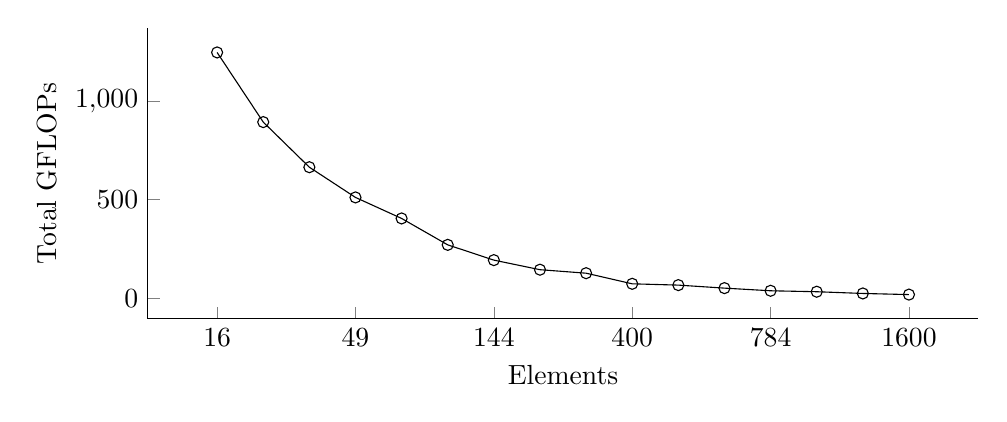
\begin{tikzpicture}
    \begin{axis}[
        height=15em,
        width=\linewidth,
        axis x line*=bottom,
        axis y line*=left,
        symbolic x coords = {16, 25, 36, 49, 64, 100, 144, 196, 225, 400, 441, 576, 784, 900, 1225, 1600},
        xtick = {16, 49, 144, 400, 784, 1600},
        ytick = {0, 500, 1000, 1500},
        domain = 16:1600,
        range = 0:1500,
        xlabel={Elements},
        ylabel={Total GFLOPs}]
        \addplot[
            mark=o,
            color=black] coordinates {
            	(16, 1244.6784)
            	(25, 892.1854771)
            	(36, 663.82848)
            	(49, 510.93504)
            	(64, 404.52048)
            	(100, 270.8420198)
            	(144, 193.61664)             	 
            	(196, 145.152) 
            	(225, 127.4550682) 
            	(400, 73.68496128) 
            	(441, 67.09248) 
            	(576, 51.8616) 
            	(784, 38.46528) 
            	(900, 33.63397632) 
            	(1225, 24.89647104)
            	(1600, 19.16804736)		
            };
    \end{axis}
\end{tikzpicture}

            

%	\captionof{figure}{Total FLOPs used to compute the factorized matrix multiplication in $\textbf{F}^{\intercal} \times (\textbf{M}^{-1} \textbf{F})$ over the number of elements for a constant problem size, $N = 705\kern 0.25em 600$. FLOPs decrease as the size of the constituent inner products decrease in relation to the size of each element.}
%\end{mcfigure}


%\begin{mcfigure}
%	\centering
%	\begin{tikzpicture}
    \begin{axis}[
        height=2.5in,
        width=3.375in,
        axis x line*=bottom,
        axis y line*=left,
        symbolic x coords = {49, 64, 100, 144, 196, 225, 400, 441, 576, 784, 900, 1225, 1600},
        xtick = {49, 144, 400, 784, 1600},
        ytick distance=20,
        domain = 49:1600,
        range = 0:60,
        xlabel={Elements},
        ylabel={Runtime (s)}]
        \addplot[dashed, 
            mark=x,
            color=violet] coordinates {
            	(49, 58.048654)
            	(64, 44.608081)
            	(100, 30.117423)
            	(144, 22.058077)             	 
            	(196, 16.56574) 
            	(225, 14.797055) 
            	(400, 9.426228) 
            	(441, 8.84558) 
            	(576, 7.915462) 
            	(784, 8.569443) 
            	(900, 9.894469) 
            	(1225, 16.662268)
            	(1600, 32.297395)		
            };                                      
        \addplot[dashed, 
            mark=triangle,
            color=blue] coordinates {
            	(49, 7.159366)
            	(64, 7.466476)
            	(100, 8.700982)
            	(144, 10.472512)             	 
            	(196, 11.721377) 
            	(225, 11.966759) 
            	(400, 14.197423) 
            	(441, 14.494765) 
            	(576, 14.587827) 
            	(784, 15.465336) 
            	(900, 15.557051) 
            	(1225, 16.686761)
            	(1600, 19.131444)		
            };
        \addplot[dashed, 
            mark=+,
            color=red] coordinates {
            	(49, 3.739837)
            	(64, 4.359711)
            	(100, 5.000516)
            	(144, 6.416801)             	 
            	(196, 8.051781) 
            	(225, 9.404944)
            	(400, 9.965406) 
            	(441, 13.815412) 
            	(576, 16.399836) 
            	(784, 19.31444) 
            	(900, 20.800298) 
            	(1225, 24.993118)
            	(1600, 29.029143)		
            };

        \addplot[
            mark=o,
            color=black] coordinates {
                (49, 69.749697)
                (64, 57.215341)
                (100, 45.317181)
                (144, 40.655649)             
                (196, 37.752682)
                (225, 36.783105)
                (400, 37.477622)
                (441, 37.671921)
                (576, 38.931754)
                (784, 43.377669)
                (900, 46.279928)
                (1225, 58.368563)
                (1600, 80.487622)
            };

        \addlegendentry{$\textbf{F}^{\intercal} \textbf{M}^{-1} \textbf{F}$}
        \addlegendentry{Style 2}
        \addlegendentry{$\lambda_A \lambda_b$}
        \addlegendentry{Total TTS}

    \end{axis}
\end{tikzpicture}
%\end{mcfigure}

